\begin{figure}
	\tikzsetnextfilename{intorno-dinfty-r2}
	\centering
	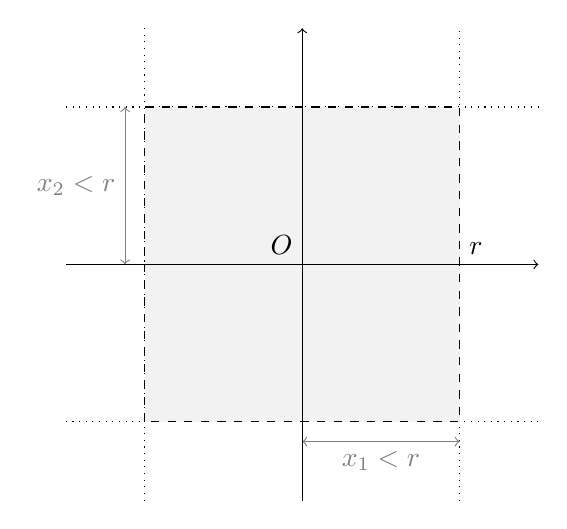
\begin{tikzpicture}
		\draw[dotted] (-3,2) -- (3,2);
		\draw[dotted] (3,-2) -- (-3,-2);
		\draw[dotted] (2,-3) -- (2,0) node[above right]{$r$};
		\draw[dotted] (2,0) -- (2,3);
		\draw[dotted] (-2,-3) -- (-2,3);
		\draw[gray,<->] (-2.25,0) to node[gray,anchor=east]{$\abs{x_2}<r$} (-2.25,2);
		\draw[gray,<->] (0,-2.25) to node[gray,anchor=north]{$\abs{x_1}<r$} (2,-2.25);
		\draw[dashed,fill=gray!10] (-2,-2) rectangle (2,2);
		\draw[->] (-3,0) -- (3,0);
		\draw[->] (0,-3) -- (0,3);
		\draw (0,0) node[anchor=south east]{$O$};
	\end{tikzpicture}
	\caption{Un intorno $B(\vec 0,r)\subset(\R^2,d_\infty)$.}
	\label{fig:B-dinfty}
\end{figure}
